\chapter{Análisis y alcance del proyecto}

\section{Análisis de requerimientos}
En general, los requerimientos hablan de lo que se espera de una aplicación, tales requerimientos se clasifican en requerimientos funcionales y no funcionales:
\begin{itemize}
\item \textbf{Requerimientos funcionales}: descripciones detalladas de las funciones deseadas del proyecto. \cite{WileyBegSE}
\item \textbf{Requerimientos no funcionales}: descripciones de la calidad y capacidades del comportamiento del proyecto. \cite{WileyBegSE}
\end{itemize}
A modo de ejemplo se muestra el caso de la generación de reportes: un requerimiento funcional habla de los datos que debe capturar un usuario para obtener un reporte (fechas de inicio y término, número de orden, etcétera), mientras que un requerimiento no funcional habla sobre el formato de salida, verificación de permisos de usuario para generar el reporte,  capacidad del sistema para atender generación simultánea de varios reportes.


\subsection{Requerimientos funcionales}
\begin{enumerate}
\item \textbf{Automatizar el proceso para contestar órdenes de reposición}. Automatizar la interacción del operador de la farmacéutica que se realiza utilizando el portal SAI para contestar las órdenes de reposición, esto implica almacenar los datos de las órdenes de reposición que son utilizados para generar el formato de salida que es entregado al almacén para continuar con la atención de las órdenes.
\item \textbf{Automatizar el proceso para cotejar órdenes de reposición canceladas}. Automatizar la interacción del operador de la farmacéutica que realizar para conocer las órdenes de reposición que han sido canceladas recientemente por el IMSS.
\item \textbf{Interfaz WEB para la administración de órdenes de reposición contestadas}. Salvo lo referente a los procesos automatizados de los operadores de la farmacéutica, todos los requerimientos de administración de órdenes de reposición y generación de reportes deben ser accedidos mediante una interfaz web protegida por nombre de usuario y contraseña. 
\item \textbf{Búsqueda de órdenes de reposición}. En la interfaz web debe existir la posibilidad de buscar entre las órdenes de reposición contestadas mediante el número de orden de reposición, esta opción entrega solo una orden de reposición, o por un intervalo de fechas entre las cuales fueron atendidas las órdenes de reposición y entrega el listado de todas las órdenes de reposición que fueron respondidas en dicho intervalo. Las órdenes resultantes de la búsqueda deben ofrecer la opción para visualizar la información almacenada durante el proceso de contestación.
\item \textbf{Edición de órdenes de reposición}. En la interfaz web debe existir la posibilidad para la edición de la información almacenada durante el proceso de respuesta de órdenes de reposición, tal edición debe ser individual, es decir, no es posible modificar más de una orden de reposición en una misma operación. El único dato que no puede ser modificado es el número de orden de reposición.
\item \textbf{Generación de reporte de órdenes de reposición contestadas}. El reporte con órdenes de reposición contestadas debe ser acotado entre fechas con precisión de horas, tal reporte, como su nombre lo indica, contiene los números de orden de reposición y datos definidos por la farmacéutica\footnote{Por acuerdo de confidencialidad no se enunciarán los datos contenidos en los reportes.} .
\item \textbf{Generación de formato de salida}. Este formato contiene datos con las órdenes de reposición y relaciones con claves de producto y centros de salud. El reporte está acotado por un intervalo de fechas con precisión de horas\footnote{Por acuerdo de confidencialidad no se enunciarán los datos contenidos en el formato de salida así como el contenido de los catálogos de claves de producto y centros de salud.}.
\item \textbf{Generación de reporte con las órdenes de reposición canceladas reciéntemente}. Genera un reporte con las órdenes de reposición canceladas recientemente, es decir, las órdenes de reposición que tienen el estado de “cancelada” y no se han marcado como canceladas en el proceso de respuesta.
\item \textbf{Actualización de estatus de órdenes de reposición canceladas}. La actualización del estatus de las órdenes de reposición canceladas quiere decir que al sistema se le ``alimenta'' de forma masiva mediante un archivo con los números de las órdenes de reposición que han sido canceladas y se ha notificado al área correspondiente de la farmacéutica para cancelar la atención de dichas órdenes.
\item \textbf{Actualización de catálogos de medicamentos}. Alimentar de forma masiva, mediante un archivo separado por comas, el catálogo con claves de medicamentos.
\end{enumerate}


\subsection{Requerimientos no funcionales}
El cliente ha solicitado que el proyecto se apegue a su infraestructura, para conservar el acuerdo de confidencialidad y evitar exponer al cliente a riesgos de seguridad informática, no se enunciarán las versiones y tipo de infraestructura utilizada:
\begin{enumerate}
\item Sistema operativo capaz de ejecutar el software Java Virtual Machine (JVM).
\item Base de datos relacional SQL.
\item Uso de la herramienta Sahi para automatizar interacción con portal web SAI.
\item Las contraseñas de los usuarios para el acceso a la interfaz web deben ser almacenadas de forma segura, es decir, cifradas mediante una función hash.
\end{enumerate}


\subsection{Alcance del Proyecto}
%definir alcance
\begin{itemize}
\item El desarrollo de automatizar el proceso para contestar órdenes de reposición inicia con la ejecución del agente.
\item Queda fuera de alcance la verificación de existencia del medicamento en bodega.
\item Queda fuera de alcance la ejecución en paralelo de más de una instancia del proceso para contestar órdenes de reposición.
\item Queda fuera de alcance la ejecución en paralelo de más de una instancia del proceso para cotejar órdenes de reposición canceladas.
\item Queda fuera del desarrollo la administración de usuarios de la interfaz WEB mediante esta misma.
\item Queda fuera de alcance la ejecución simultánea de los procesos para contestar órdenes de reposición y cotejar órdenes de reposición canceladas.
\item Queda fuera de alcance la realización de respaldos de la información contenida en la base de datos o en el sistema de archivos.
\end{itemize}


\subsection{Riesgos asociados al proyecto}
%definir riesgos
\begin{itemize}
\item Al no contar con un ambiente de pruebas del portal SAI todos los datos alterados durante la programación de las rutinas de automatización podrían persistir información incorrecta, entonces es necesario mantener siempre un registro de las órdenes de reposición alteradas durante el desarrollo de las rutinas de automatización.
\item La herramientas de automatización se sustentan en la estructura DOM de las páginas HTML por las que navegan, entonces si ocurriera un cambio en dicha estructura las rutinas de automatización podrían dejar de funcionar.
\item El uso de software libre no tiene garantía por lo cual se reconoce como riesgo el fallo de software desarrollado por terceros.
\end{itemize}


\section{Casos de uso}
Un caso de uso es la representación de las posibles interacciones entre el sistema y sus actores, entendiendo un actor como una instancia (usuario u otro sistema). Así mismo, un caso de uso describe la funcionalidad del sistema por medio de mensajes y respuestas entre el actor y el sistema\cite{ApressSE}.\\
En las siguientes descripciones de caso de uso no se hará referencia al contenido exacto de las páginas así como el nombre de los campos, únicamente se hará mención de los campos necesarios para dar una explicación clara del caso.

\begin{figure}[h]
\centering
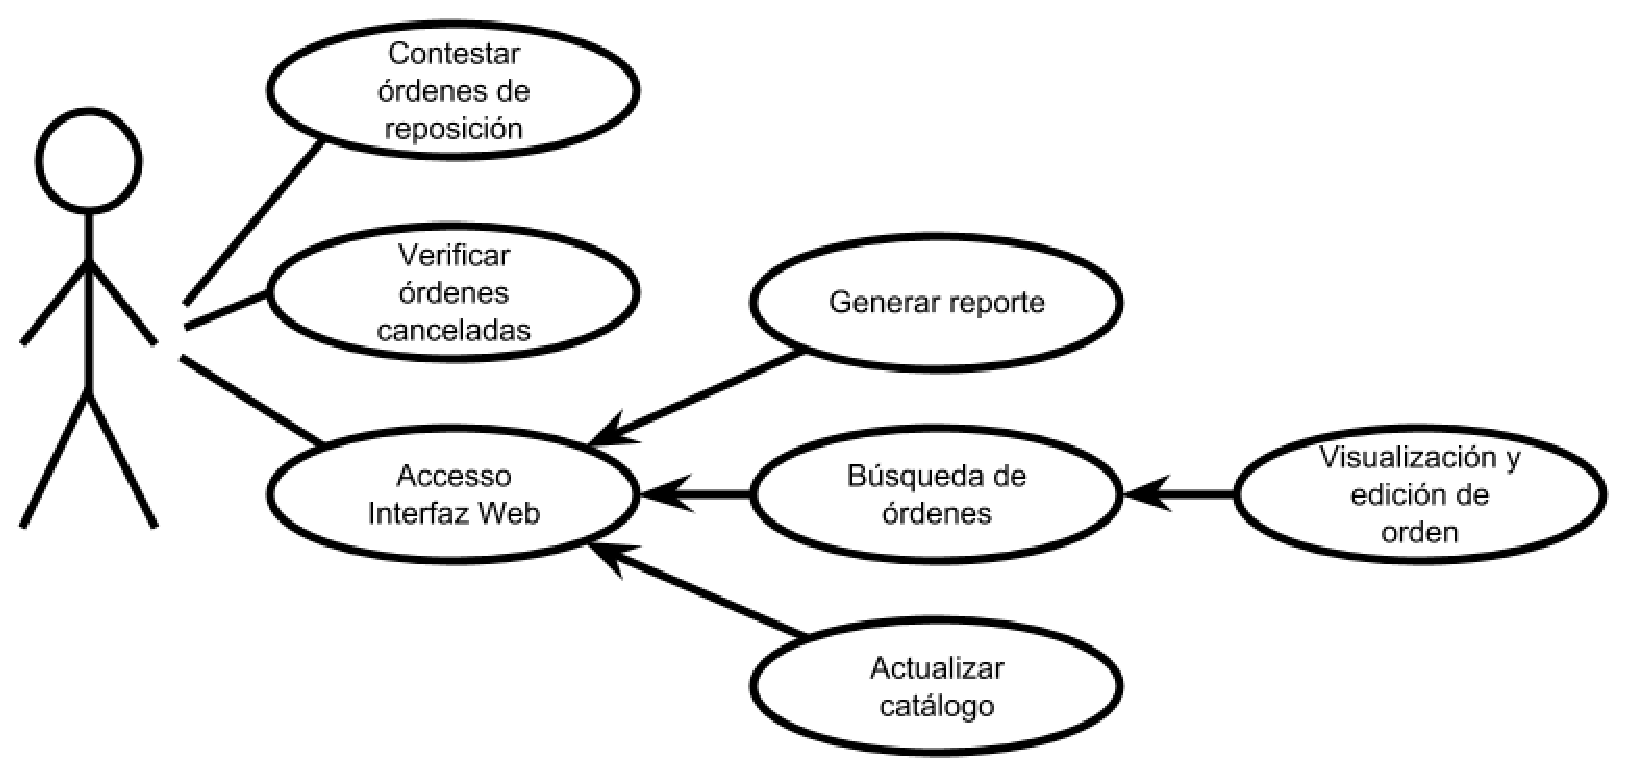
\includegraphics[width=\textwidth]{dia-casos-uso} 
\caption{Diagrama de casos de uso.}
\label{fig:dia-casos-uso}
\end{figure}


\subsection{Contestar órdenes de reposición}
\paragraph{Identificador}
CU1
\paragraph{Actores}
Usuario
\paragraph{Descripción}
\paragraph{Precondiciones}
\paragraph{Secuencia normal}
\begin{enumerate}
  \item Inicia sesión en portal SAI: provee nombre de usuario y le solicita al usuario ingresar la contraseña.
  \item Dirige el explorador a la pantalla donde se encuentra el listado con las órdenes de reposición que no han sido contestadas.
  \item Del listado de órdenes de reposición, ingresa al sistema las primeras 20 (procesamiento por lotes); cada solicitud es ingresada a la base de datos con estatus \textbf{Nueva} y datos provenientes del listado:
  \begin{enumerate}
    \item Contrato.
    \item Solicitud.
    \item Número de orden.
    \item Fecha de expedición.
    \item Almacén destino.
    \item \textit{URL} de contestación.
    \item \textit{URL} de envío:
    \begin{enumerate}
      \item Si el listado muestra este dato, entonces el estatus cambia a \textbf{Contestada} y se registra la \textbf{cantidad solicitada} en 0;
      \item Si no se encuentra, entonces se genera reemplazando el parámetro en la \textit{URL} de contestación ``responde'' por ``envia''.
    \end{enumerate}
  \end{enumerate}
  \item Para cada solicitud con estatus \textbf{Nueva}:
  \begin{enumerate}
    \item Cambia el estatus a \textbf{Siendo Contestada}.
    \item Dirige el explorador a la \textit{URL} de contestación obtenida en el paso 3-f.
    \item Llena el formulario que se presenta en esta pantalla con las siguientes consideraciones:
    \begin{enumerate}
      \item Fecha de fabricación: primer día del año en curso si la fecha actual no es del mes de diciembre, en caso contrario se toma el año siguiente.
      \item Fecha de caducidad: último día del año en curso si la fecha actual no es del mes de diciembre, en caso contrario se toma el año siguiente.
    \end{enumerate}
    \item En la base de datos se almacenan los datos de las tablas de la pantalla actual.
    \item Si no ha ocurrido ningún error, el estatus cambia a \textbf{Contestada}; en caso contrario, el estatus cambia a \textbf{Error}.
  \end{enumerate}
  \item Para cada solicitud con estatus \textbf{Contestada}:
  \begin{enumerate}
  \item Cambia estatus a \textbf{Siendo Enviada}.
  \item El explorador dirige a la \textit{URL de envío}.
  \item Ejecutar caso de uso CU9.
  \item Si no ha ocurrido ningún error, el estatus cambia a \textbf{Enviada}; en caso contrario, el estatus cambia a \textbf{Error}.
  \item El programa se repite desde el paso 2 hasta terminar las solicitudes sin contar las marcadas con estatus \textbf{Error}.
  \end{enumerate}
  \item Registra el fin del procedimiento en la base de datos.
\end{enumerate}
\paragraph{Postcondiciones}
\paragraph{Excepciones}


\subsection{Verificar órdenes de reposición canceladas}
\paragraph{Identificador}
CU2
\paragraph{Actores}
Usuario
\paragraph{Descripción}
\paragraph{Precondiciones}
\paragraph{Secuencia normal}
\begin{enumerate}
  \item Inicia sesión en portal SAI: provee nombre de usuario y le solicita al usuario ingresar la contraseña.
  \item Dirige el explorador a la pantalla de búsqueda de órdenes de reposición.
  \item Llena el formulario para el filtro de búsqueda:
  \begin{enumerate}
    \item Rango de fechas que comprende los últimos 3 días desde la fecha actual.
    \item Estado \textbf{Cancelada}.
  \end{enumerate}
  \item Del listado de órdenes de reposición resultantes genera una lista con el número de orden de cada renglón.
  \item Actualiza el estado SAI de las órdenes de reposición en la base de datos.
\end{enumerate}
\paragraph{Postcondiciones}
\paragraph{Excepciones}


\subsection{Acceso a interfaz Web}
\paragraph{Identificador}
CU3
\paragraph{Actores}
Usuario
\paragraph{Descripción}
\paragraph{Precondiciones}
\paragraph{Secuencia normal}
\begin{enumerate}
  \item El sistema muestra la pantalla de acceso.
  \item El usuario ingresa los campos:
  \begin{enumerate}
    \item Nombre de usuario.
    \item Contraseña.
  \end{enumerate}
  \item El sistema busca el nombre de usuario en la base de datos
  \item El sistema compara la contraseña provista en el paso 1.b con el valor almacenado en la base de datos.
  \item Muestra la pantalla de generación de reportes.
\end{enumerate}
\paragraph{Postcondiciones}
\paragraph{Excepciones}
\begin{enumerate}
  \item En los siguientes esceneracios se concideran un error de autencación.
  \begin{itemize}
    \item El usuario no existe en la base de datos.
    \item El usuario tiene estado \textbf{deshabilitado}.
    \item La contraseña proporcionada no coincide con la almacenada. 
  \end{itemize}
\end{enumerate}

\subsection{Generación de reportes}
\paragraph{Identificador}
CU4
\paragraph{Actores}
Usuario
\paragraph{Descripción}
\paragraph{Precondiciones}
\paragraph{Secuencia normal}
\begin{enumerate}
  \item En la pantalla de generación de reportes el usuario realiza las siguientes acciones:
    \begin{enumerate}
    \item Llenar el formulario de la pantalla con los siguientes campos:
    \begin{enumerate}
      \item \textbf{Tipo de reporte}
      \item \textbf{Fecha y hora inicial}
      \item \textbf{Fecha y hora final}
    \end{enumerate}
    \item Enviar el formulario.
  \end{enumerate}
  \item El sistema ejecuta los siguientes pasos:
  \begin{enumerate}
    \item Realiza para consulta a la base de datos definida para el reporte requerido en 1.a.
    \item El resultado del paso anterior es escrito en un archivo extendido de Excel y depositado en el sistema de archivos.
    \item Muestra al usuario la ruta en el sistema de archivos donde fue depositado el reporte.
  \end{enumerate}
\end{enumerate}
\paragraph{Postcondiciones}
\paragraph{Excepciones}


\subsection{Actualización de catálogos}
\paragraph{Identificador}
CU5
\paragraph{Actores}
Usuario
\paragraph{Descripción}
\paragraph{Precondiciones}
\paragraph{Secuencia normal}
\begin{enumerate}
  \item El usuario realiza las siguientes acciones en la pantalla de administración de catálogos:
  \begin{enumerate}
    \item Seleccionar el nombre del catálogo.
    \item Seleccionar el archivo en formato de Excel que contiene la información para el catálogo.
    \item Enviar el formulario.
  \end{enumerate}
  \item El sistema sigue los siguientes pasos:
  \begin{enumerate}
    \item Valida el formato del archivo recibido.
    \item Valida que el archivo recibido contenga al menos un renglón sin contar el encabezado.
    \item Borra el contenido del catálogo en la base datos y copia la información del archivo recibido.
    \item Muestra al usuario el número de registros guardados en el catálogo después de la actualización.
  \end{enumerate}
\end{enumerate}
\paragraph{Postcondiciones}
\paragraph{Excepciones}


\subsection{Búsqueda de órdenes de reposición}
\paragraph{Identificador}
CU6
\paragraph{Actores}
Usuario
\paragraph{Descripción}
\paragraph{Precondiciones}
\paragraph{Secuencia normal}
\begin{enumerate}
  \item El usuario realiza los siguientes pasos:
  \begin{enumerate}
    \item Capturar los criterios para la búsqueda presentados en el filtro:
    \begin{enumerate}
      \item Número de orden.
      \item Estatus de atención.
      \item Rango de fechas en que fueron atendidas las órdenes de reposición.
    \end{enumerate}
  \end{enumerate}
  \item El sistema muestra el resultado de la búsqueda, para cada orden de reposición listada se muestra un enlace que lleva a la visualización y edición de la orden (ver casos de uso Visualización y Edición de orden de reposición).

\end{enumerate}
\paragraph{Postcondiciones}
\paragraph{Excepciones}


\subsection{Visualización de orden de reposición}
\paragraph{Identificador}
CU7
\paragraph{Actores}
Usuario
\paragraph{Descripción}
\paragraph{Precondiciones}
\paragraph{Secuencia normal}
\begin{enumerate}
  \item El usuario selecciona la orden reposición del listado de búsqueda (ver caso de uso búsqueda de órdenes de reposición).
  \item Se muestra la pantalla con los datos de la orden.
  \begin{enumerate}
    \item Se muestran todos los datos capturados del portal SAI durante el procedimiento de atención.
    \item También se muestran los estados de atención, es decir el estado en el portal SAI  y el estado de atención.
  \end{enumerate}
\end{enumerate}
\paragraph{Postcondiciones}
\paragraph{Excepciones}


\subsection{Edición de orden de reposición}
\paragraph{Identificador}
CU8
\paragraph{Actores}
Usuario
\paragraph{Descripción}
\paragraph{Precondiciones}
\paragraph{Secuencia normal}
\begin{enumerate}
\item Modificar cualquiera de los campos editables (ver caso de uso visualización de orden de reposición).
\item Seleccionar el botón Guardar.
\item Opcionalmente se puede volver a general el documento PDF seleccionado en el botón PDF.
\end{enumerate}
\paragraph{Postcondiciones}
\paragraph{Excepciones}


\subsection{Generar captura de pantalla de envío}
\paragraph{Identificador}
CU9
\paragraph{Actores}
Usuario
\paragraph{Descripción}
\paragraph{Precondiciones}
\paragraph{Secuencia normal}
\begin{enumerate}
\item 
\end{enumerate}
\paragraph{Postcondiciones}
\paragraph{Excepciones}
